\section{Methodology}\label{sec:methods}

\subsection{Theoretical Foundations}\label{subsec:theory}

The Kolmogorov complexity $K(x)$ is defined as the length of the
shortest program that produces the binary string $x$ on a Universal
Turing machine \cite{li2004similarity}. Because $K(x)$ is uncomputable,
practical applications approximate it via lossless compression.
The Normalized Information Distance (NID) \cite{li2004similarity} is

\begin{equation}
  \mathrm{NID}(x,y)
  = \frac{\max\bigl\{K(x\mid y),\,K(y\mid x)\bigr\}}
         {\max\bigl\{K(x),\,K(y)\bigr\}},
  \label{eq:nid}
\end{equation}

\noindent where $x$ and $y$ are arbitrary binary strings;
$K(x \mid y)$ is the conditional Kolmogorov complexity of $x$
given $y$ (length of the shortest program producing $x$ with $y$
as auxiliary input); $K(y \mid x)$ is defined symmetrically; and
$\max\{K(x), K(y)\}$ normalises the distance to $[0,1]$.

Its computable approximation, the Normalized Compression Distance
(NCD) \cite{cilibrasi2005clustering}, replaces $K$ with the output length $C_z(\cdot)$
of lossless compressor $z$:

\begin{equation}
  \mathrm{NCD}_z(x,y)
  = \frac{C_z(xy) - \min\bigl\{C_z(x),\,C_z(y)\bigr\}}
         {\max\bigl\{C_z(x),\,C_z(y)\bigr\}},
  \label{eq:ncd}
\end{equation}

\noindent where $xy$ is the concatenation of strings $x$ and $y$;
$C_z(x)$ and $C_z(y)$ are their individually compressed lengths
(bytes) under algorithm $z \in \mathcal{Z} = \{\texttt{gzip},
\texttt{zlib}, \texttt{bz2}\}$; $C_z(xy)$ is the joint compressed
length; and $\mathrm{NCD}_z \in [0,1+\varepsilon]$ with
$\varepsilon \to 0$ as compressor quality improves \cite{cilibrasi2005clustering}.

The Compression-based Dissimilarity Measure (CDM) \cite{keogh2007compression}
provides a complementary formulation:

\begin{equation}
  \mathrm{CDM}_z(x,y)
  = \frac{C_z(xy)}{C_z(x) + C_z(y)},
  \label{eq:cdm}
\end{equation}

\noindent where all symbols are as in Eq.~\eqref{eq:ncd}. NCD
emphasises marginal compression gain, whereas CDM expresses the
ratio of joint to summed compressed lengths: two metrics that
capture complementary aspects of informational overlap.

The Compression Length Measure (CLM)\cite{jiang2022fewshot}
\revadd{complements the previous formulations through a
length-normalised expression}:

\begin{equation}
  \mathrm{CLM}_z(x,y)
  = \frac{1 - \bigl(C_z(x) + C_z(y) - C_z(xy)\bigr)}
         {C_z(xy)},
  \label{eq:clm}
\end{equation}

\noindent \revadd{where all symbols are as in Eq.~\eqref{eq:ncd}; the numerator
rewards joint compressibility by quantifying the residual between the
summed individual compressed lengths and the joint compressed length,
while the denominator normalises by the joint length. In the experiments
reported below, the full metric family
$\mathcal{M} = \{\mathrm{NCD}, \mathrm{CDM}, \mathrm{CLM}\}$ is exposed
to the search procedure, and the best-performing subset per dataset is
selected on the search split}.

\subsection{Pipeline Overview}\label{subsec:pipeline}

The SCoPE prediction pipeline comprises four sequential stages:
(1) support-set construction; (2) dissimilarity matrix computation;
(3) geometric feature extraction and distance scoring;
(4) ensemble voting.

\subsection{Stage 1: Support-Set Construction}\label{subsec:stage1}

Let $\mathcal{D} = \{(m_i, y_i)\}_{i=1}^{N}$ with $m_i$ a
\revmod{SMILES string (without canonicalisation)} and
$y_i \in \{0,1\}$. A support set
$\mathcal{S}_c$ for candidate class $c \in \{0,1\}$ is drawn from
the 30\% search partition:

\begin{equation}
  \mathcal{S}_c = \bigl\{m_j : y_j = c,\;
                 j \in \mathcal{I}_{\mathrm{search}}\bigr\},
  \quad |\mathcal{S}_c| = k,
  \label{eq:support}
\end{equation}

\noindent where $k$ is selected via grid search on the search split
and $\mathcal{I}_{\mathrm{search}}$ is the index set of the search
partition. The binary flag \texttt{keep\_similar} controls whether the
self-similarity entries---the diagonal elements of the pairwise matrix,
where a string is compared with itself---are retained
(\texttt{keep\_similar}=\texttt{True}) or omitted
(\texttt{keep\_similar}=\texttt{False}). When retained, the matrix gains
one additional feature column per comparison (the query-to-query and
support-to-support entries), enlarging the feature dimensionality from
$k$ to $k+1$; when omitted, the diagonal is skipped.
\revmod{Here and below we write $p = k + 1$ when
\texttt{keep\_similar}=\texttt{True} and $p = k$ otherwise, to denote
the per-row feature dimensionality of the dissimilarity matrices, which
therefore depends on \texttt{keep\_similar}.}
Both settings are
explored by the search procedure. This is an implementation-level
feature-selection decision \revmod{over the dimensionality of the
dissimilarity representation} rather than a similarity threshold on the
support set.

\subsection{Stage 2: Dissimilarity Matrix Computation}\label{subsec:stage2}

For each class $c$, compressor $z$, and metric
$d \in \mathcal{M}$, a matrix
\revmod{$\mathbf{M}^{(z,d)}_c \in
\mathbb{R}^{(k+1)\times p}$} is
computed over $\hat{\mathcal{S}}_c = \mathcal{S}_c \cup \{m_q\}$,
\revmod{where $p$ is the per-row feature dimensionality defined above
($p = k+1$ with \texttt{keep\_similar}=\texttt{True}, $p = k$
otherwise), so the matrix has $k+1$ rows---one per support string plus
the query---and $p$ retained comparison columns}:

\begin{equation}
  \left[\mathbf{M}^{(z,d)}_c\right]_{ij}
  = d_z(s_i,\, s_j),
  \quad s_i,\, s_j \in \hat{\mathcal{S}}_c,
  \label{eq:matrix}
\end{equation}

\noindent where $d_z$ is \revmod{one of} $\mathrm{NCD}_z$, $\mathrm{CDM}_z$, \revmod{or $\mathrm{CLM}_z$};
$s_i, s_j$ are SMILES strings indexed $1$ to $k+1$; index
$k+1$ is reserved for $m_q$; \revmod{and when
\texttt{keep\_similar}=\texttt{False} the self-comparison entries
($s_i$ versus itself) are dropped from the columns}. The complete set
of matrices is

\begin{equation}
  \mathbb{M}_c = \bigl\{\mathbf{M}^{(z,d)}_c :\;
                z \in \mathcal{Z},\;
                d \in \mathcal{M}\bigr\},
  \label{eq:matrixset}
\end{equation}

yielding $|\mathcal{Z}| \times |\mathcal{M}|$ matrices per class per
query.
gzip and zlib implement Lempel-Ziv-77 coding (short-range pattern
matching); bz2 applies Burrows-Wheeler block sorting followed by
Huffman coding, capturing long-range SMILES dependencies
unavailable to Lempel-Ziv schemes \cite{keogh2007compression}.

\begin{figure}[H]
    \centering
    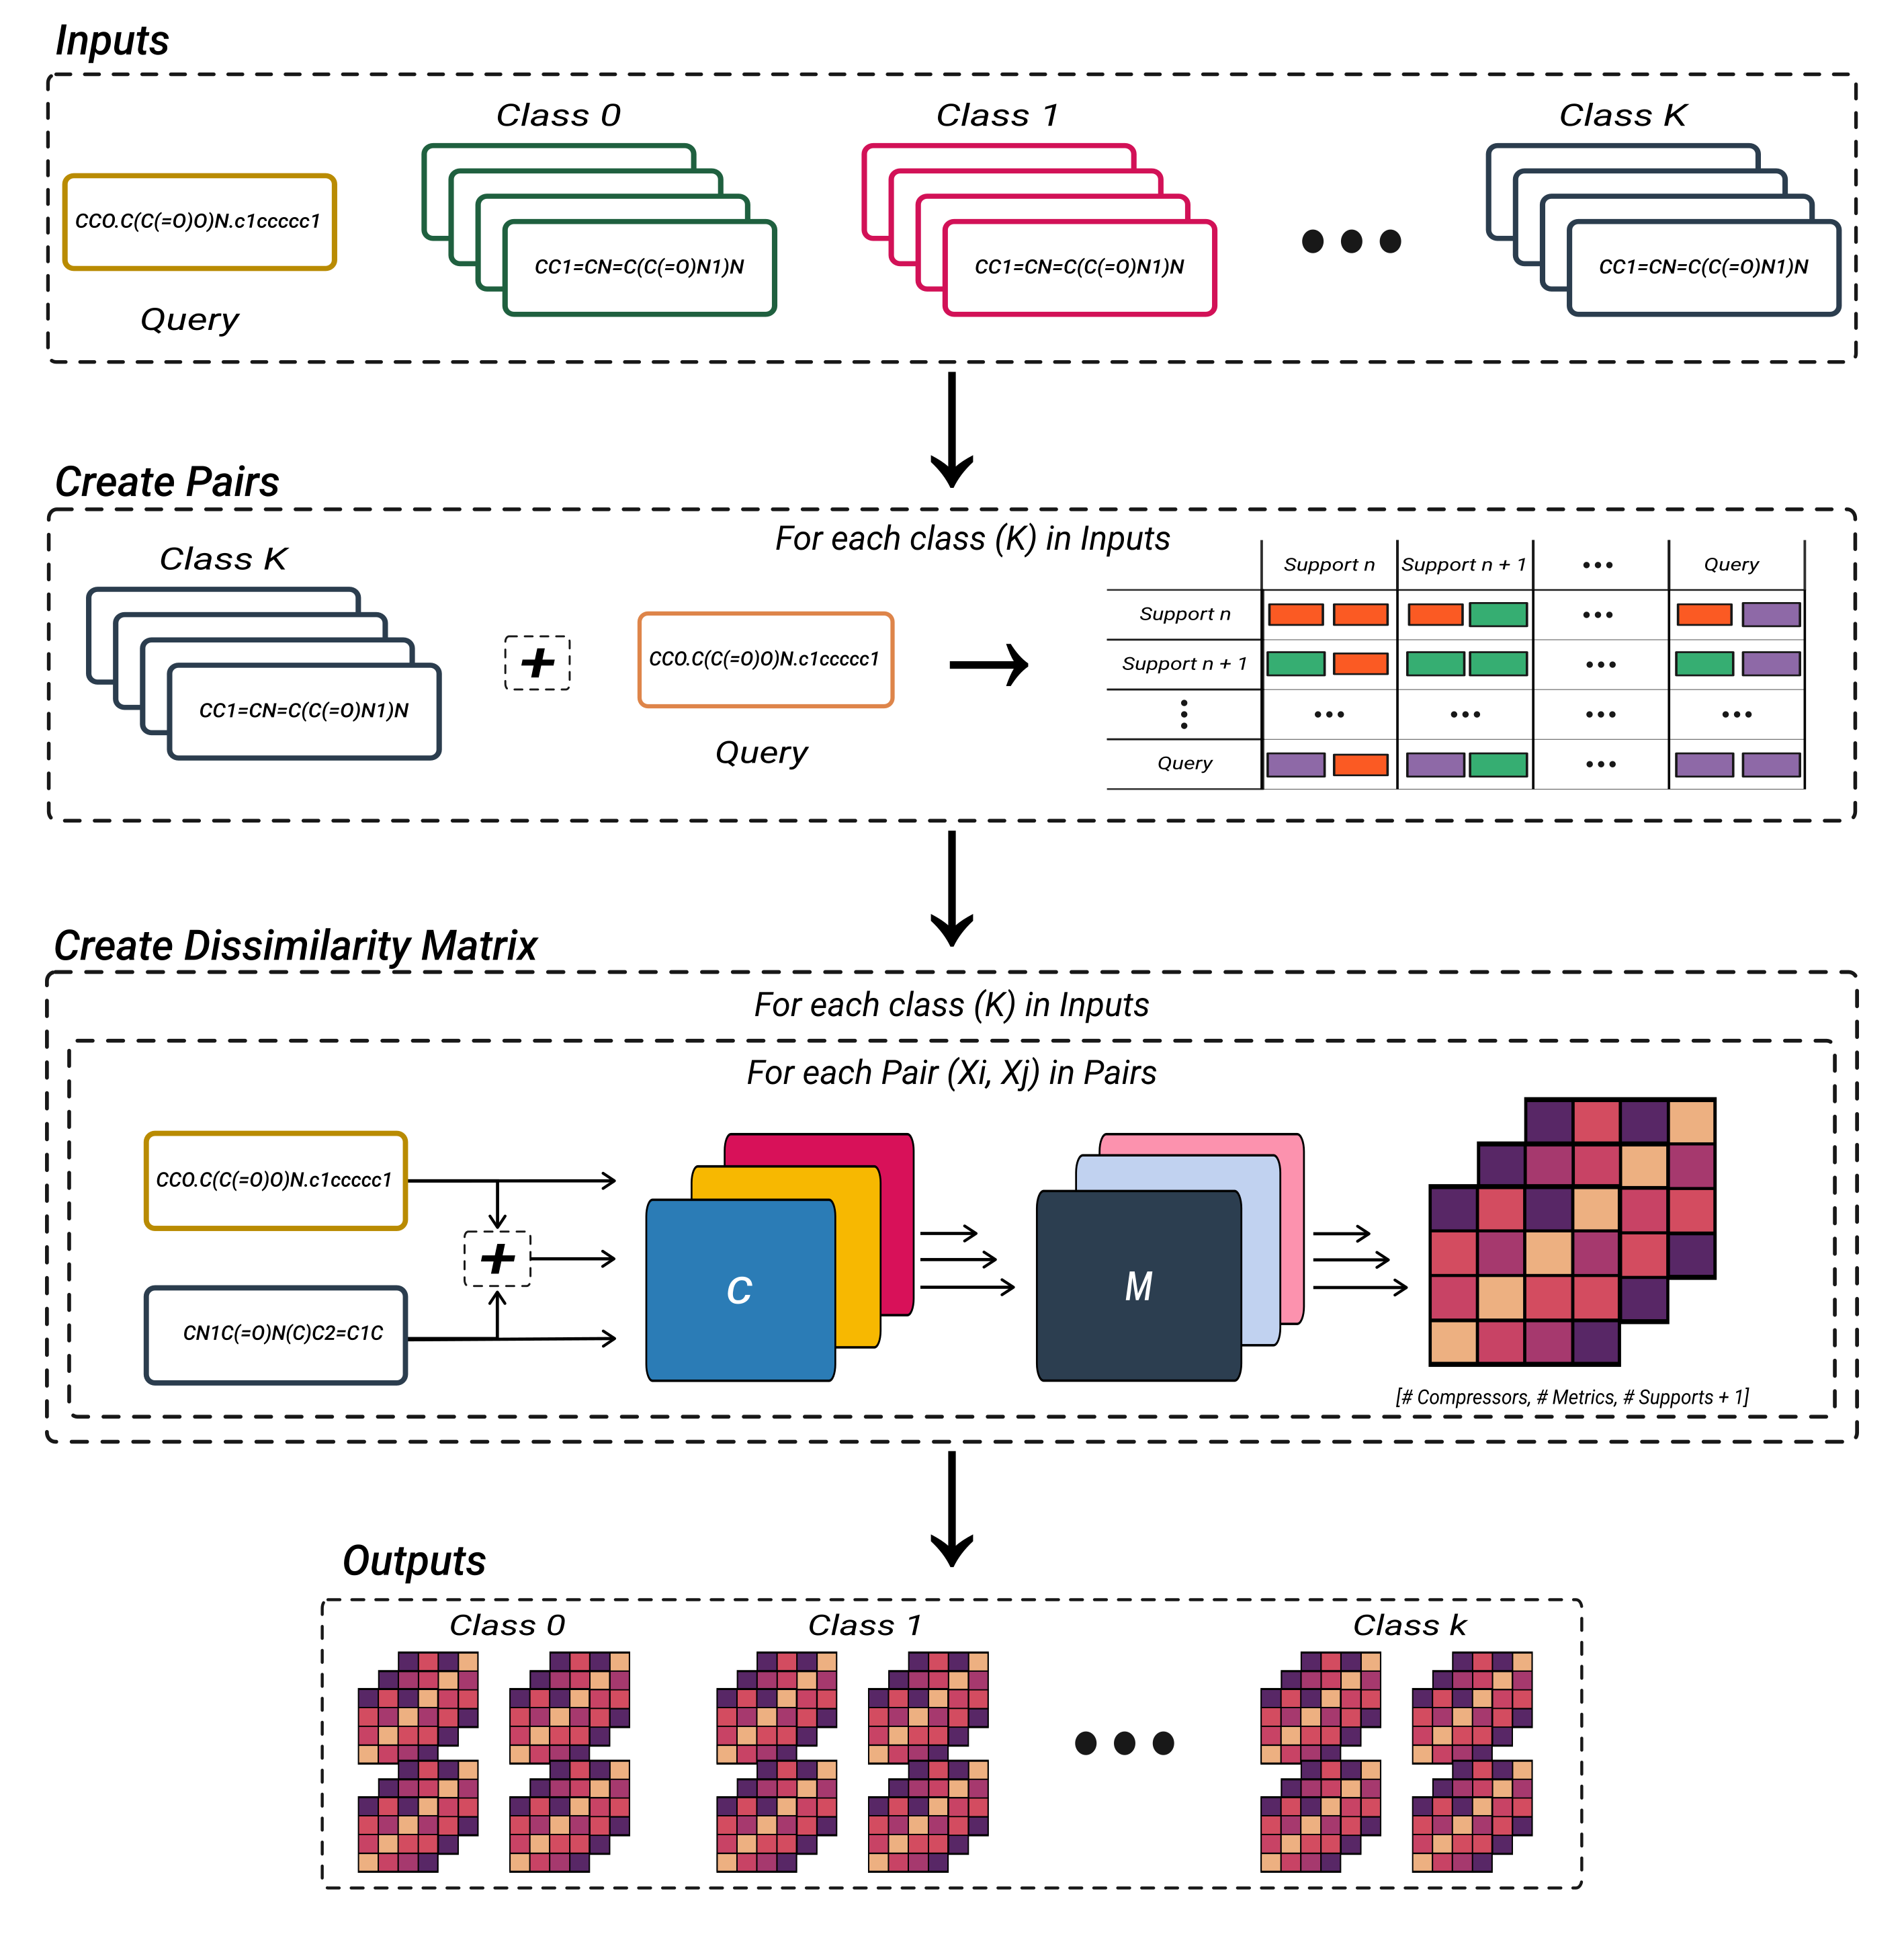
\includegraphics[width=0.8\columnwidth]{images/workflow/dm.png}
    \caption{Overview of the dissimilarity matrix computation stage in SCoPE. The process illustrates the separation of query and class SMILES strings, the construction of the combined support-query matrices, and the pairwise evaluation across compressors ($C$) and metrics ($M$).}
    \label{fig:dissimilarity_matrix}
\end{figure}

\subsection{Stage 3: Geometric Feature Extraction}\label{subsec:stage3}

The support centroid is the mean row vector over the $k$ support
members:

\begin{equation}
  \boldsymbol{\mu}_c^{(z,d)}
  = \frac{1}{k}\sum_{i=1}^{k} \mathbf{M}^{(z,d)}_c[i,\,:],
  \label{eq:centroid}
\end{equation}

\noindent where $\mathbf{M}^{(z,d)}_c[i,\,:]$ is the $i$-th row
\revmod{(dimension $p$)}; and $\boldsymbol{\mu}_c^{(z,d)} \in
\revmod{\mathbb{R}^{p}}$ encodes the mean dissimilarity profile of class
$c$. The query feature vector is

\begin{equation}
  \mathbf{q}_c^{(z,d)}
  = \mathbf{M}^{(z,d)}_c[k+1,\,:],
  \label{eq:query}
\end{equation}

\noindent where $k+1$ is the reserved query index, and
$\mathbf{q}_c^{(z,d)} \in \revmod{\mathbb{R}^{p}}$ encodes the
dissimilarity of $m_q$ to every augmented-support element.
\revmod{Two distance factors are computed from these vectors and
combined multiplicatively into the scoring distance;}
the individual factors are then collapsed into the product
(Eq.~\eqref{eq:combined}):

\paragraph{Euclidean distance}
\begin{equation}
  d_{\mathrm{E}}(\boldsymbol{\mu},\mathbf{q})
  = \|\boldsymbol{\mu} - \mathbf{q}\|_2
  = \sqrt{\sum_{l=1}^{\revmod{p}}(\mu_l - q_l)^2},
  \label{eq:euclidean}
\end{equation}
where $\mu_l, q_l$ are the $l$-th components and the sum runs over
\revmod{all $p$ dimensions} of the feature vectors. Euclidean distance is sensitive to absolute
magnitude differences.

\paragraph{Cosine distance}
\begin{equation}
  d_{\mathrm{C}}(\boldsymbol{\mu},\mathbf{q})
  = 1 - \frac{\boldsymbol{\mu} \cdot \mathbf{q}}
             {\|\boldsymbol{\mu}\|_2\,\|\mathbf{q}\|_2},
  \label{eq:cosine}
\end{equation}
where $\boldsymbol{\mu} \cdot \mathbf{q}$ is the inner product and
$\|\cdot\|_2$ is the Euclidean norm. Cosine distance captures
angular separation independently of vector magnitudes, providing
invariance to compression-ratio differences across molecule sizes.

\paragraph{Combined distance}
\begin{equation}
  d_{\mathrm{X}}(\boldsymbol{\mu},\mathbf{q})
  = d_{\mathrm{E}}(\boldsymbol{\mu},\mathbf{q})
    \times
    d_{\mathrm{C}}(\boldsymbol{\mu},\mathbf{q}),
  \label{eq:combined}
\end{equation}
where $d_{\mathrm{E}}$ and $d_{\mathrm{C}}$ are as in
Eqs.~\eqref{eq:euclidean} and \eqref{eq:cosine}. The product
amplifies consensus: when both metrics simultaneously assign low
distance to a class, $d_{\mathrm{X}}$ is especially small;
disagreement penalises the product, encoding an implicit confidence
requirement.

\subsection{Stage 4: Ensemble Voting}\label{subsec:stage4}

For each compressor--metric pair $(z, d)$, a base classifier votes
\revmod{on the combined distance} $d_{\mathrm{X}}$
(Eq.~\eqref{eq:combined}):

\begin{equation}
  v^{(z,d)}
  = \underset{c\,\in\,\{0,1\}}{\arg\min}\;
    d_{\mathrm{X}}\!\left(\boldsymbol{\mu}_c^{(z,d)},\;
               \mathbf{q}_c^{(z,d)}\right),
  \label{eq:vote}
\end{equation}

\noindent where $v^{(z,d)} \in \{0,1\}$ selects the class whose
centroid is closest to the query under that compressor--metric
combination. \revmod{Note that the Euclidean and cosine distances are
computed internally, but the decision rests exclusively on their
product}; no base classifier votes on either factor independently.
This produces $|\mathcal{Z}| \times |\mathcal{M}|$ base votes. The
final prediction is

\begin{equation}
  \hat{y}_q
  = \underset{c\,\in\,\{0,1\}}{\arg\max}\;
    \sum_{z,d}
    \mathbf{1}\!\left[v^{(z,d)} = c\right],
  \label{eq:majority}
\end{equation}

\noindent where $\mathbf{1}[\cdot]$ is the indicator function and
the double sum aggregates \revmod{all $|\mathcal{Z}| \times
|\mathcal{M}|$ votes}. \revmod{In ties, the smallest class index is
selected, consistent with the \texttt{argmax} over the vote-count
vector.}

\begin{figure}[H]
    \centering
    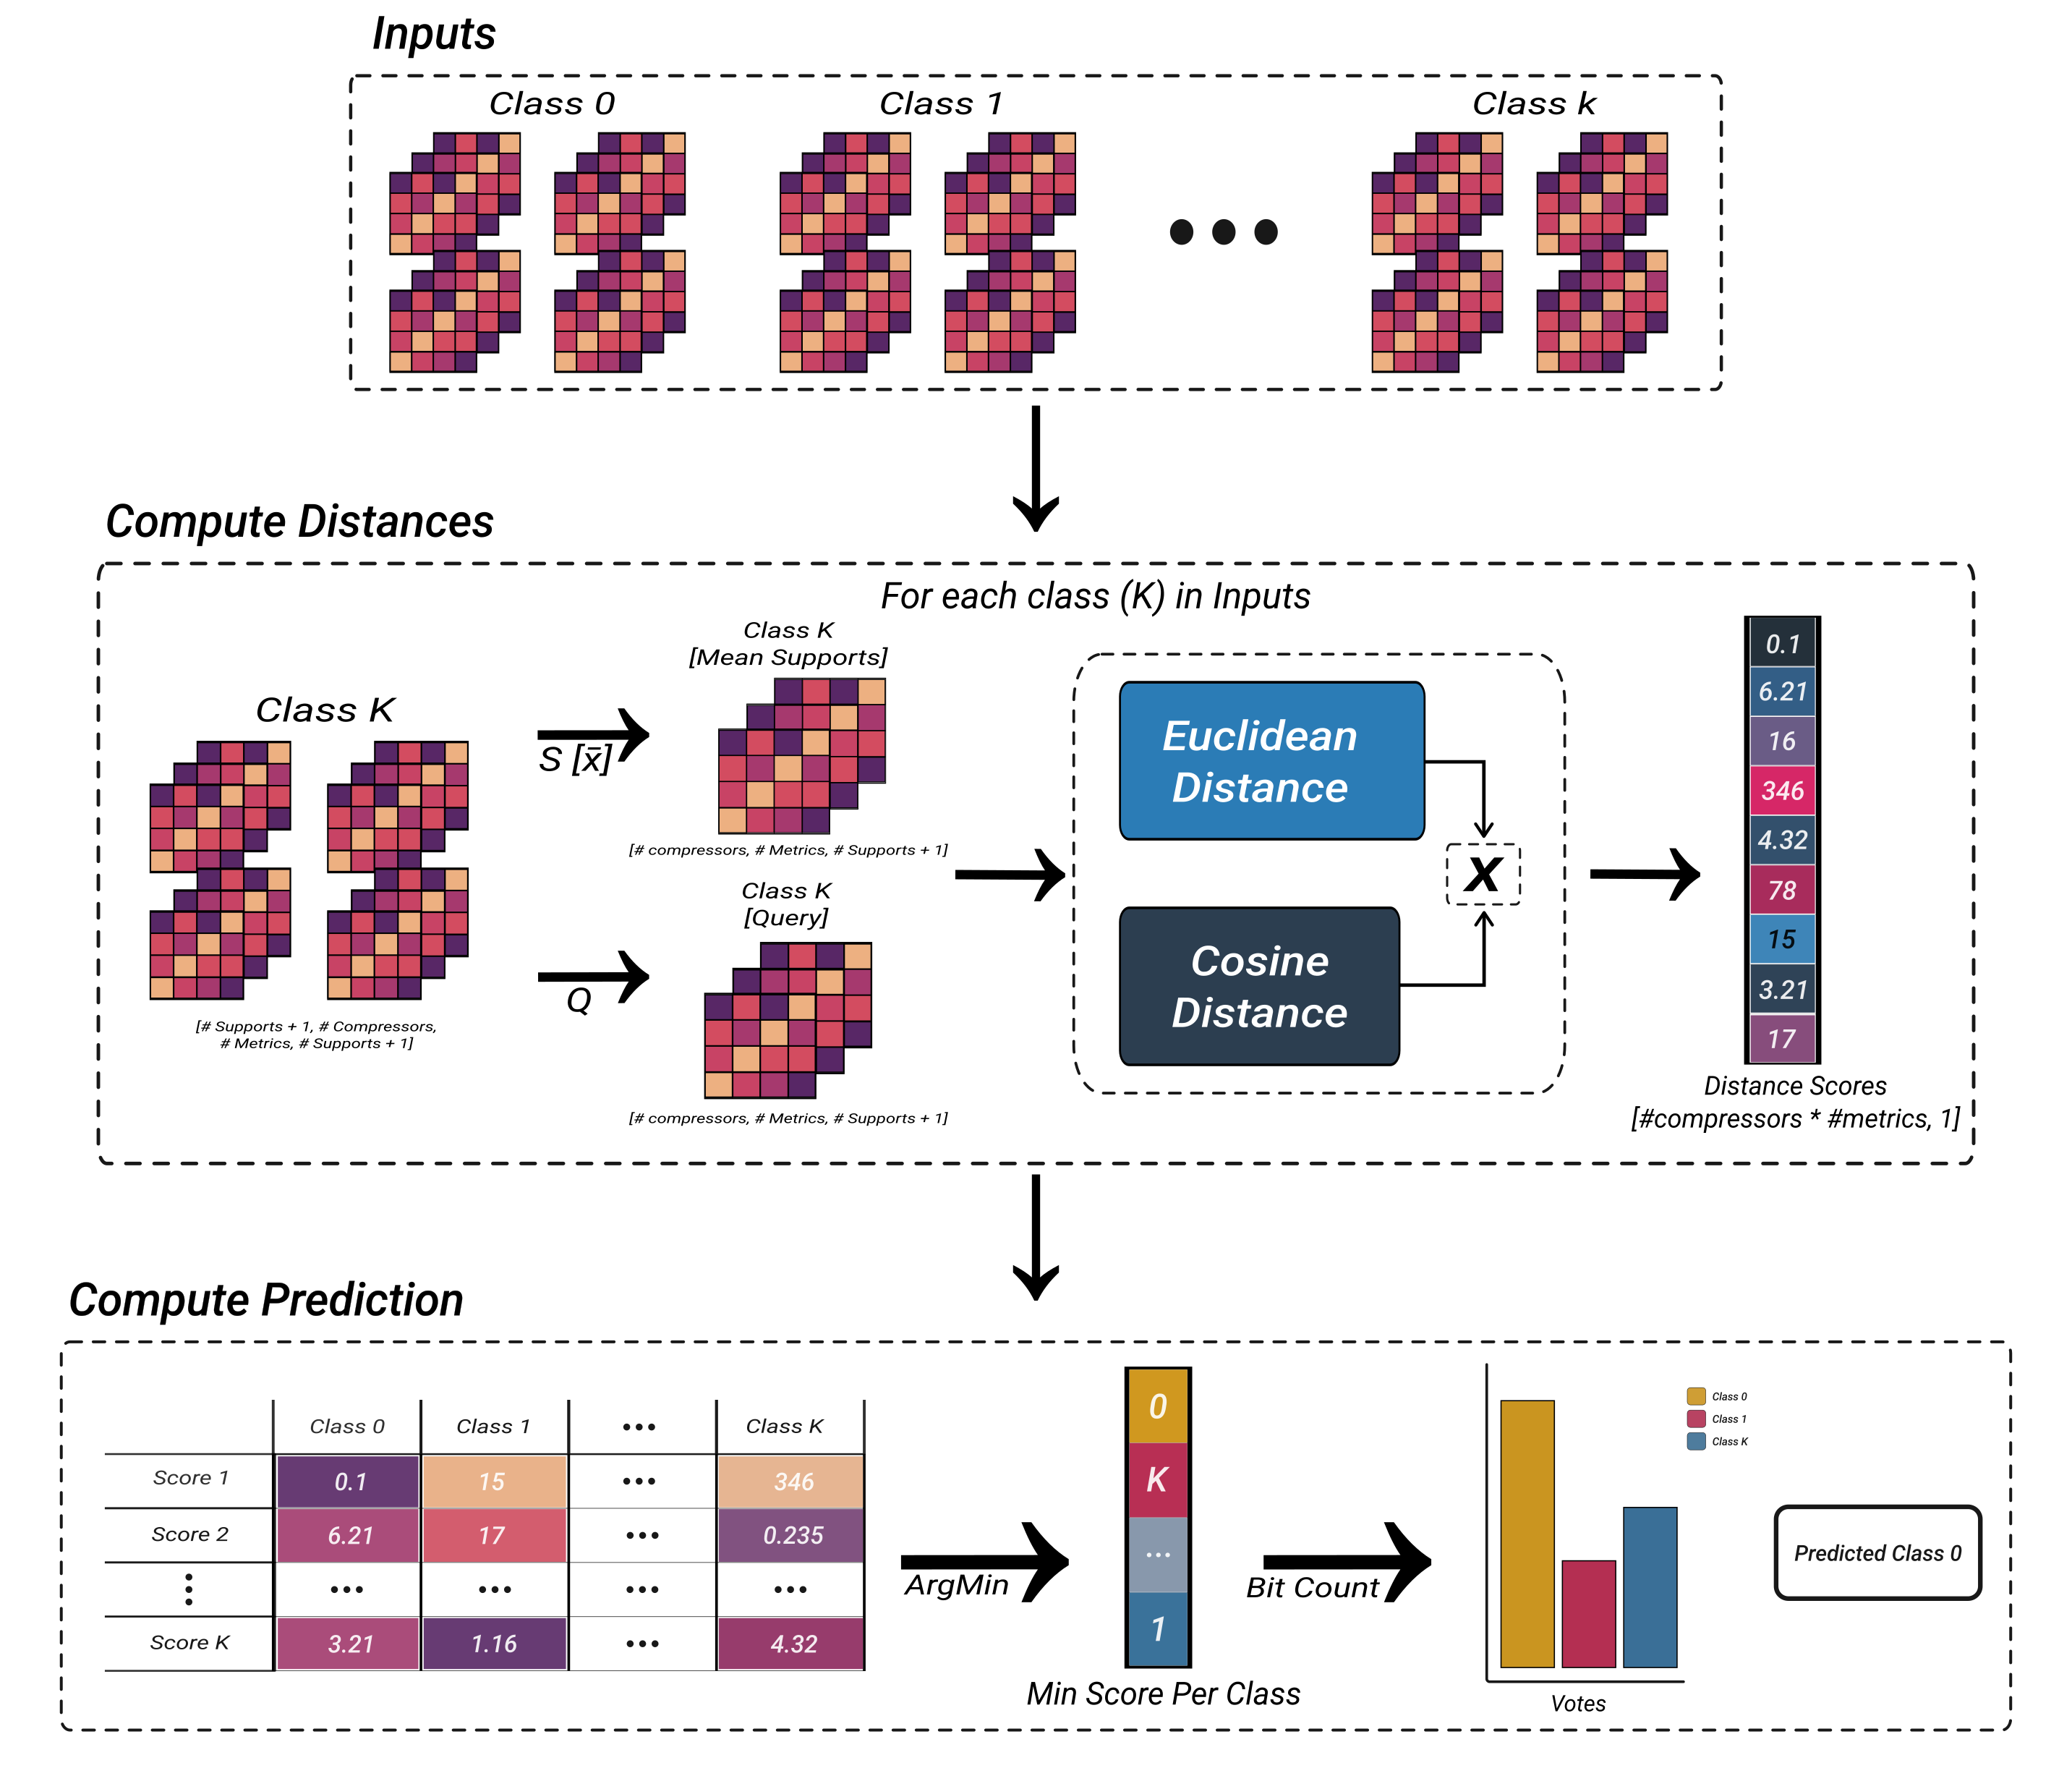
\includegraphics[width=0.8\columnwidth]{images/workflow/prediction.png}
    \caption{Geometric feature extraction and ensemble voting pipeline. Upper and middle sections depict the extraction of class centroids ($\mu$) and query vectors ($q$), alongside the combined Euclidean and cosine distance scoring. The bottom section illustrates the $\text{ArgMin}$ selection, bit/vote counting, and final majority-vote class prediction.}
    \label{fig:scope_workflow}
\end{figure}

\subsection{Parameter Search and Experimental Protocol}\label{subsec:params}

\revmod{The exhaustive grid search considers three hyperparameters: the
compressor set $\mathcal{C}$, the dissimilarity-metric set $\mathcal{M}$,
and the \texttt{keep\_similar} flag, which can take either
$\mathrm{True}$ or $\mathrm{False}$. The sets $\mathcal{C}$ and
$\mathcal{M}$ can be any non-empty subsets of
$\{\texttt{bz2}, \texttt{zlib}, \texttt{gzip}\}$ and
$\{\mathrm{NCD}, \mathrm{CDM}, \mathrm{CLM}\}$, respectively.
Thus, a configuration can use either a single compressor--metric
combination or multiple combinations. In the latter case, each
compressor--metric pair contributes one feature to the dissimilarity
matrix; each feature votes for the class whose support centroid lies
closest to the query, and the final prediction is determined by majority
voting. This results in $7 \times 7 \times 2 = 98$ candidate
configurations.}

\revmod{Each configuration is evaluated under two protocols governing the
support-set size $k$. In the \emph{fixed} protocol, $k$ is held
constant across all queries and takes one of the values in
$\{3, 5, 8, 10, 15, 17, 20\}$. In the \emph{variable} protocol,
designed to assess robustness under non-stationary conditions, $k$
is randomly sampled from the integer range $[3, 20]$ independently
for each query, allowing the number of support examples to vary
across queries.}

\revmod{The optimization objective is balanced accuracy on the 30\% search
split, averaged over five stratified folds. The best-performing
configuration is subsequently evaluated on the 70\% test split,
which remains strictly isolated from the model-selection process.
Under the variable protocol, the support-set size for each test
query is also independently sampled from the same range, ensuring
that the test evaluation follows the same variability assumption
without reusing the search-split samples.}

\revmod{Finally, the experiments use a random (non-scaffold) 70/30
partition. Comparisons with methods based on scaffold splits or
80/10/10 partitioning should therefore be interpreted in light of
this methodological difference} (see Section~\ref{subsec:compare}).

\subsection{Datasets}\label{subsec:data}

All experiments used three benchmark datasets from MoleculeNet
\cite{wu2018moleculenet}. \textbf{ClinTox} \cite{gayvert2016datadriven} comprises 1,478
compounds annotated for clinical trial toxicity and FDA approval
status; the positive (toxic) class accounts for approximately 8\%
of instances, making it highly imbalanced. The drugs considered as
toxic were originally obtained from the AACT database, while those
approved were obtained from DrugBank 4.0, providing a robust
framework for evaluating structure-toxicity relationships
\cite{gayvert2016datadriven}. \textbf{BBBP} \cite{martins2012bayesian} contains 2,053 compounds
annotated for blood-brain barrier penetration; the dataset was
compiled from multiple publications and curated to resolve
annotation inconsistencies \cite{martins2012bayesian}. \textbf{BACE} \cite{subramanian2016computational}
contains 1,513 compounds with binary BACE-1 binding inhibition
\revmod{labels; the binary activity label (Class) is used as target.
All molecules are represented by the SMILES strings} \cite{weininger1988smiles}
\revmod{without further canonicalisation, sanitisation, or
featurisation.}

\revadd{As preprocessing, the loading stage ignores SMILES strings
shorter than 30 characters before the 70/30 test/search partition.}
